\subsubsection{\NonOptimizing MSVC}

\RU{Вот что выдал MSVC 2010}\EN{MSVC 2010 generated}:

\lstinputlisting[caption=MSVC 2010]{patterns/12_FPU/3_comparison/x86/MSVC/\LANG.asm}

\index{x86!\Instructions!FLD}
\RU{Итак, \FLD загружает \TT{\_b} в регистр \ST{0}.}
\EN{So, \FLD loading \TT{\_b} into the \ST{0} register.}

\label{Czero_etc}
\newcommand{\Czero}{\TT{C0}\xspace}
\newcommand{\Ctwo}{\TT{C2}\xspace}
\newcommand{\Cthree}{\TT{C3}\xspace}
\newcommand{\CThreeBits}{\Cthree/\Ctwo/\Czero}

\index{x86!\Instructions!FCOMP}
\RU{\FCOMP сравнивает содержимое \ST{0} с тем что лежит в \TT{\_a} и выставляет биты \CThreeBits в 
регистре статуса FPU. Это 16-битный регистр отражающий текущее состояние FPU.} 
\EN{\FCOMP compares the value in the \ST{0} register with what is in \TT{\_a} value 
and set \CThreeBits bits in FPU 
status word register. 
This is 16-bit register reflecting current state of FPU.} 

\RU{Итак, биты \CThreeBits выставлены, но, к сожалению, у процессоров до Intel P6 
\footnote{Intel P6 это Pentium Pro, Pentium II, и далее} нет инструкций условного перехода,
проверяющих эти биты. 
Возможно, так сложилось исторически (вспомните о том что FPU когда-то был вообще отдельным чипом). 
А у Intel P6 появились инструкции \FCOMI/\FCOMIP/\FUCOMI/\FUCOMIP ~--- делающие тоже самое, 
только напрямую модифицирующие флаги \ZF/\PF/\CF.}
\EN{For now \CThreeBits bits are set, but unfortunately, CPU before Intel P6
\footnote{Intel P6 is Pentium Pro, Pentium II, etc} has not any conditional 
jumps instructions which are checking these bits. 
Probably, it is a matter of history (remember: FPU was separate chip in past). 
Modern CPU starting at Intel P6 has \FCOMI/\FCOMIP/\FUCOMI/\FUCOMIP 
instructions~---which does the same, but modifies CPU flags \ZF/\PF/\CF.}

\RU{После этого, инструкция \FCOMP выдергивает одно значение из стека. 
Это отличает её от \FCOM, которая просто сравнивает значения, оставляя стек в таком же состоянии.}
\EN{After bits are set, the \FCOMP instruction popping one variable from stack. 
This is what distinguish it from \FCOM, which is just comparing values, leaving the stack at the same state.}

\index{x86!\Instructions!FNSTSW}
\RU{\FNSTSW копирует содержимое регистра статуса в \AX. Биты \CThreeBits занимают позиции, 
соответственно, 14, 10, 8, в этих позициях они и остаются в регистре \AX, 
и все они расположены в старшей части регистра ~--- \AH.}
\EN{\FNSTSW copies FPU status word register to the \AX. Bits \CThreeBits are placed at positions 14/10/8, 
they will be at the same positions in the \AX register and all they are placed in high part of the \AX{}~---\AH{}.}

\begin{itemize}
\item
\RU{Если b>a в нашем случае, то биты \CThreeBits должны быть выставлены так:}
\EN{If b>a in our example, then \CThreeBits bits will be set as following:} 0, 0, 0.
\item
\RU{Если a>b, то биты будут выставлены:}\EN{If a>b, then bits will be set:} 0, 0, 1.
\item
\RU{Если a=b, то биты будут выставлены так:}\EN{If a=b, then bits will be set:} 1, 0, 0.
\end{itemize}
% TODO: table here?

\RU{После исполнения \TT{test ah, 5}, бит \Cthree и \TT{C1} сбросится в ноль, 
на позициях 0 и 2 (внутри регистра \AH) 
останутся соответственно \Czero и \Ctwo.}
\EN{After \TT{test ah, 5} execution, bits \Cthree and \TT{C1} will be set to 0, 
but at positions 0 and 2 (in the \AH registers) 
\Czero and \Ctwo bits will be left.}

\label{parity_flag}
\index{x86!\Registers!\RU{Флаг четности}\EN{Parity flag}}
\RU{Теперь немного о \IT{parity flag}\footnote{флаг четности}. Еще один замечательный рудимент}
\EN{Now let's talk about parity flag. Another notable epoch rudiment}:

\begin{framed}
\begin{quotation}
One common reason to test the parity flag actually has nothing to do with parity. The FPU has four condition flags 
(C0 to C3), but they can not be tested directly, and must instead be first copied to the flags register. 
When this happens, C0 is placed in the carry flag, C2 in the parity flag and C3 in the zero flag. 
The C2 flag is set when e.g. incomparable floating point values (NaN or unsupported format) are compared 
with the FUCOM instructions.\footnote{\url{http://en.wikipedia.org/wiki/Parity_flag}}
\end{quotation}
\end{framed}

\RU{Этот флаг выставляется в $1$ если количество единиц в последнем результате ~--- четно. 
И в $0$ если ~--- нечетно.}
\EN{This flag is to be set to $1$ if ones number is even. And to $0$ if odd.}

\index{x86!\Instructions!JP}
\RU{Таким образом, что мы имеем, флаг \PF будет выставлен в $1$, если \Czero и \Ctwo 
оба $1$ или оба $0$. 
И тогда сработает последующий \JP (\IT{jump if PF==1}). 
Если мы вернемся чуть назад и посмотрим значения \CThreeBits 
для разных вариантов, то увидим, что условный переход \JP сработает в двух случаях: если b>a или если a==b 
(ведь бит \Cthree уже \IT{вылетел} после исполнения \TT{test ah, 5}).}
\EN{Thus, \PF flag will be set to 1 if both \Czero and \Ctwo are set to $0$ or both are $1$.
And then following \JP (\IT{jump if PF==1}) will be triggered. 
If we recall values of the \CThreeBits for various cases,
we will see the conditional jump 
\JP will be triggered in two cases: if b>a or a==b 
(\Cthree bit is already not considering here since it was cleared while execution of 
the \TT{test ah, 5} instruction).}

\RU{Дальше все просто. Если условный переход сработал, то \FLD загрузит значение \TT{\_b} в \ST{0}, 
а если не сработал, то загрузится \TT{\_a} и произойдет выход из функции.}
\EN{It is all simple thereafter. If conditional jump was triggered, \FLD will load the \TT{\_b} value 
to the \ST{0} register, and if it is not triggered, the value of the \TT{\_a} variable will be loaded.}

\paragraph{\RU{Первый пример с \olly}\EN{First \olly example}: a=1.2 \AndENRU b=3.4}

\RU{Загружаем пример в}\EN{Let's load the example into} \olly: \figref{fig:FPU_comparison_case1_olly1}.
\RU{Текущие параметры ф-ции}\EN{Current function arguments are}: $a=1.2$ \AndENRU $b=3.4$ 
(\RU{их видно в стеке: 2 пары 32-битных значений}\EN{We can see them in stack: two pairs of 32-bit values}).
\IT{b} ($3.4$) \RU{уже загружено в}\EN{already loaded in} \ST{0}.
\RU{Сейчас будет исполняться \FCOMP}\EN{\FCOMP will be executed now}. 
\olly \RU{показывает второй аргумент для \FCOMP, который сейчас находится в стеке}\EN{show the second \FCOMP
argument, which is in stack right now}.\\
\\
\FCOMP \RU{отработал}\EN{executed}: \figref{fig:FPU_comparison_case1_olly2}.
\RU{Мы видим состояния condition-флагов \ac{FPU}}\EN{We see \ac{FPU} condition flags state}: 
\RU{все нули}\EN{all zeroes}.
\RU{Вытолкнутое значение перемещается в \ST{7}, почему это так, я писал раннее}
\EN{Popped value is moved into \ST{7}, I wrote earlier about reason of this}: 
\ref{FPU_is_rather_circular_buffer}.\\
\\
\FNSTSW \RU{сработал}\EN{executed}: \figref{fig:FPU_comparison_case1_olly3}.
\RU{Видно что регистр \TT{AX} содержит нули: действительно, ведь все condition-флаги тоже содержали нули.}
\EN{We see that \TT{AX} register contain zeroes: indeed, all condition flags has zeroes.}
(\olly \RU{дизассемблирует команду}\EN{disassembles} \FNSTSW \RU{как}\EN{instruction as} \TT{FSTSW} --- 
\RU{это синоним}\EN{they are synonyms}).\\
\\
\TEST \RU{сработал}\EN{executed}: \figref{fig:FPU_comparison_case1_olly4}.
\RU{Флаг \TT{PF} равен единице.}\EN{\TT{PF} flag is one.}
\RU{Все верно: количество выставленных бит в $0$ это $0$, а $0$ --- это четное число.}
\EN{Indeed: count of bits set in $0$ is $0$ and $0$ is even number.}
\olly \RU{дизассемблирует}\EN{disassembles} \TT{JP} \RU{как}\EN{as} \ac{JPE} --- \RU{это синонимы}\EN{they
are synonims}.
\RU{И она сейчас сработает}\EN{And it will be triggered right now}.\\
\\
\ac{JPE} \RU{сработала}\EN{triggered}, \FLD \RU{загрузила в \ST{0} значение \IT{b} ($3.4$)}
\EN{loads \IT{b} ($3.4$) value into \ST{0}}: \figref{fig:FPU_comparison_case1_olly5}.
\RU{Ф-ция заканчивает свою работу}\EN{The function finishes its work}.

\begin{figure}[H]
\centering
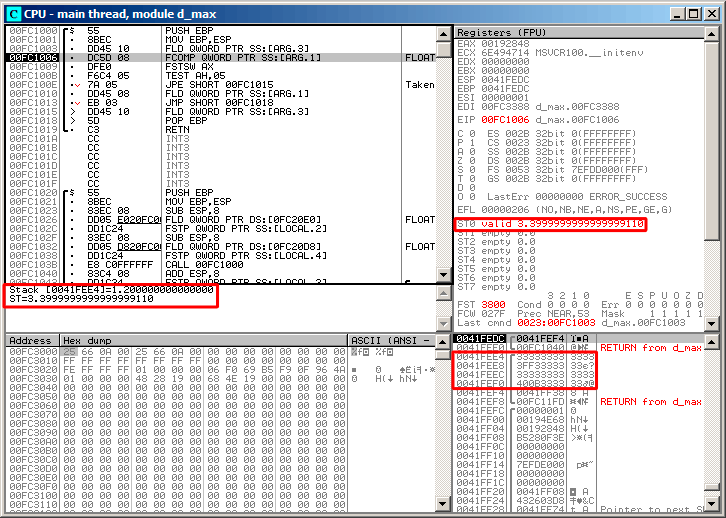
\includegraphics[scale=\FigScale]{patterns/12_FPU/3_comparison/x86/MSVC/olly1_1.png}
\caption{\olly: \RU{первая \FLD исполнилась}\EN{first \FLD executed}}
\label{fig:FPU_comparison_case1_olly1}
\end{figure}

\begin{figure}[H]
\centering
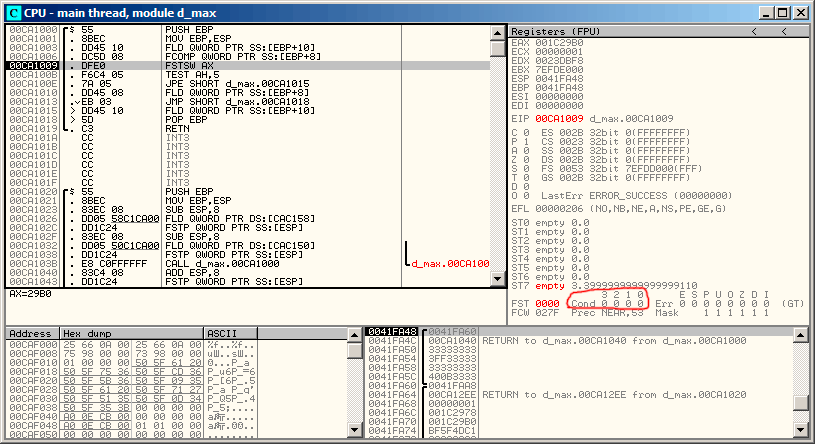
\includegraphics[scale=\FigScale]{patterns/12_FPU/3_comparison/x86/MSVC/olly1_2.png}
\caption{\olly: \FCOMP \RU{исполнилась}\EN{executed}}
\label{fig:FPU_comparison_case1_olly2}
\end{figure}

\begin{figure}[H]
\centering
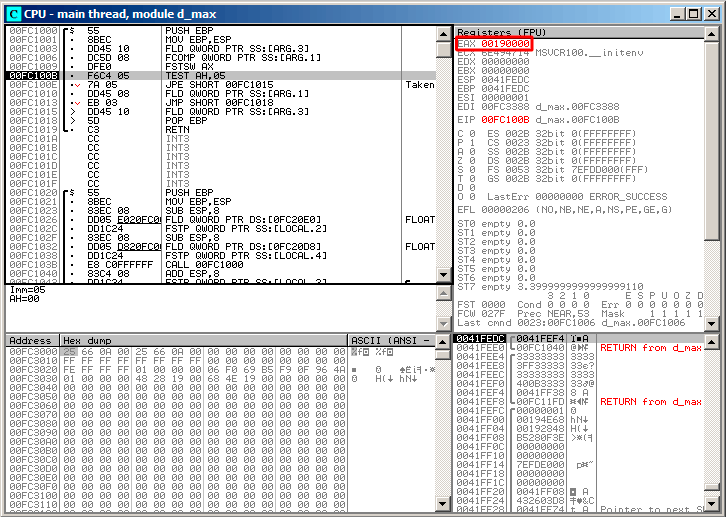
\includegraphics[scale=\FigScale]{patterns/12_FPU/3_comparison/x86/MSVC/olly1_3.png}
\caption{\olly: \FNSTSW \RU{исполнилась}\EN{executed}}
\label{fig:FPU_comparison_case1_olly3}
\end{figure}

\begin{figure}[H]
\centering
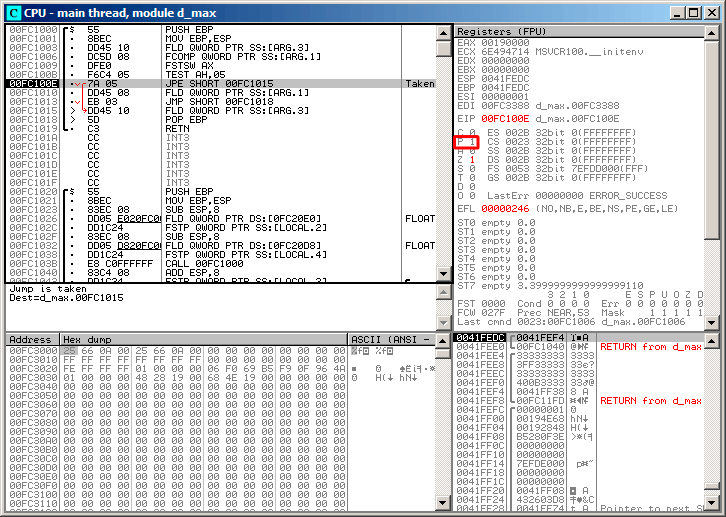
\includegraphics[scale=\FigScale]{patterns/12_FPU/3_comparison/x86/MSVC/olly1_4.png}
\caption{\olly: \TEST \RU{исполнилась}\EN{executed}}
\label{fig:FPU_comparison_case1_olly4}
\end{figure}

\begin{figure}[H]
\centering
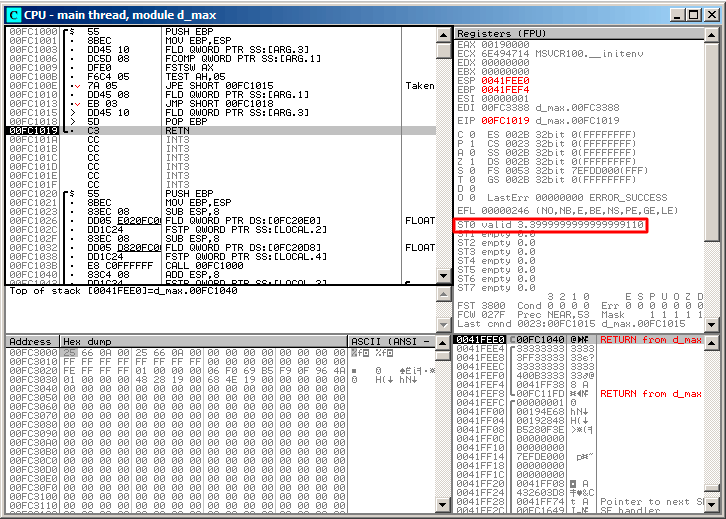
\includegraphics[scale=\FigScale]{patterns/12_FPU/3_comparison/x86/MSVC/olly1_5.png}
\caption{\olly: \RU{вторая \FLD исполнилась}\EN{second \FLD executed}}
\label{fig:FPU_comparison_case1_olly5}
\end{figure}

\paragraph{\RU{Второй пример с \olly}\EN{Second \olly example}: a=5.6 \AndENRU b=-4}

\RU{Загружаем пример в}\EN{Let's load example into} \olly: \figref{fig:FPU_comparison_case2_olly1}.
\RU{Текущие параметры ф-ции}\EN{Current function arguments are}: $a=5.6$ \AndENRU $b=-4$).
\IT{b} ($-4$) \RU{уже загружено в}\EN{is already loaded into} \ST{0}.
\RU{Сейчас будет исполняться \FCOMP}\EN{\FCOMP will be executed now}. 
\olly \RU{показывает второй аргумент \FCOMP, который сейчас находится в стеке}
\EN{shows second \FCOMP argument which is in stack right now}.\\
\\
\FCOMP \RU{отработал}\EN{executed}: \figref{fig:FPU_comparison_case2_olly2}.
\RU{Мы видим значения condition-флагов \ac{FPU}: все нули кроме \Czero.}
\EN{We see \ac{FPU} condition flags state: all zeroes except of \Czero.}\\
\\
\FNSTSW \RU{сработал}\EN{executed}: \figref{fig:FPU_comparison_case2_olly3}.
\RU{Видно что регистр \TT{AX} содержит \TT{0x100}: флаг \Czero стал на место 16-го бита.}
\EN{We see that \TT{AX} register contain \TT{0x100}: \Czero flag now on the place of 16th bit.}\\
\\
\TEST \RU{сработал}\EN{executed}: \figref{fig:FPU_comparison_case2_olly4}.
\RU{Флаг }\TT{PF} \RU{равен нулю}\EN{ flag is cleared}.
\RU{Все верно}\EN{Indeed}: 
\RU{количество единичных бит в \TT{0x100} --- это $1$, а $1$ --- это нечетное число}
\EN{count of bits set in \TT{0x100} is $1$ and $1$ is odd number}.
\ac{JPE} \RU{сейчас не сработает}\EN{will not be triggered now}.\\
\\
\ac{JPE} \RU{не сработала}\EN{wasn't triggered}, \FLD 
\RU{загрузила в \ST{0} значение \IT{a} ($5.6$)}
\EN{loads \IT{a} value ($5.6$) into \ST{0}}: \figref{fig:FPU_comparison_case2_olly5}.
\RU{Ф-ция заканчивает свою работу}\EN{The function finishes its work}.

\begin{figure}[H]
\centering
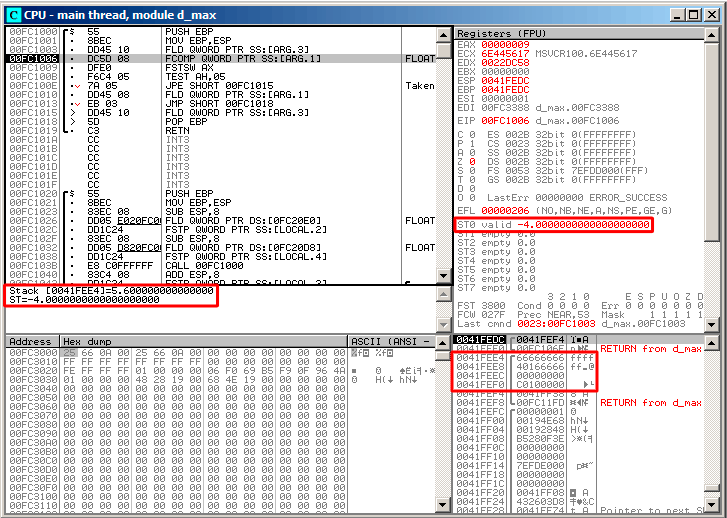
\includegraphics[scale=\FigScale]{patterns/12_FPU/3_comparison/x86/MSVC/olly2_1.png}
\caption{\olly: \RU{первая \FLD исполнилась}\EN{first \FLD executed}}
\label{fig:FPU_comparison_case2_olly1}
\end{figure}

\begin{figure}[H]
\centering
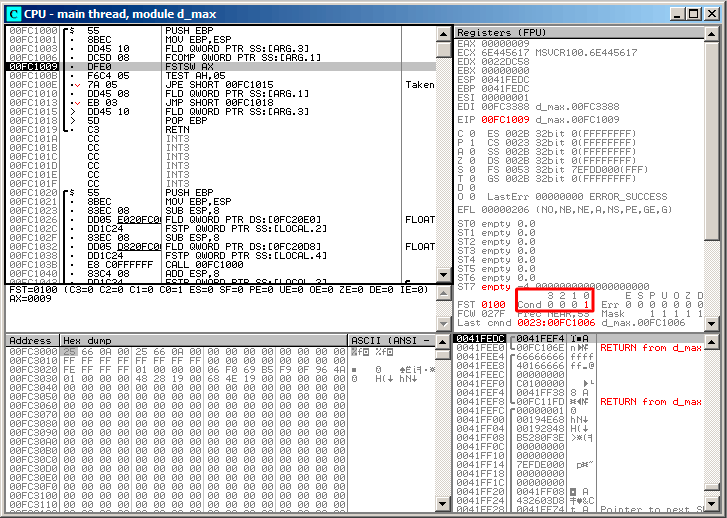
\includegraphics[scale=\FigScale]{patterns/12_FPU/3_comparison/x86/MSVC/olly2_2.png}
\caption{\olly: \FCOMP \RU{исполнилась}\EN{executed}}
\label{fig:FPU_comparison_case2_olly2}
\end{figure}

\begin{figure}[H]
\centering
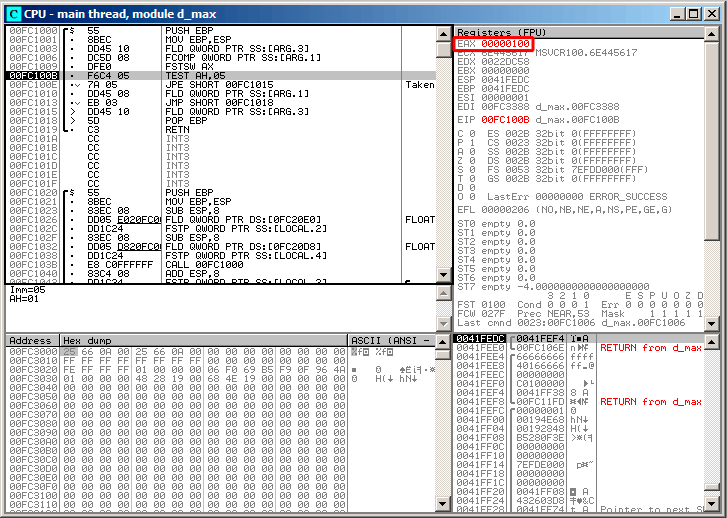
\includegraphics[scale=\FigScale]{patterns/12_FPU/3_comparison/x86/MSVC/olly2_3.png}
\caption{\olly: \FNSTSW \RU{исполнилась}\EN{executed}}
\label{fig:FPU_comparison_case2_olly3}
\end{figure}

\begin{figure}[H]
\centering
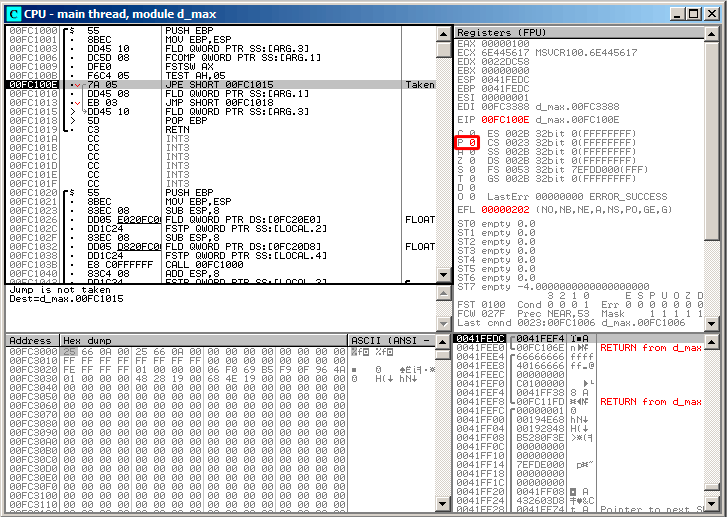
\includegraphics[scale=\FigScale]{patterns/12_FPU/3_comparison/x86/MSVC/olly2_4.png}
\caption{\olly: \TEST \RU{исполнилась}\EN{executed}}
\label{fig:FPU_comparison_case2_olly4}
\end{figure}

\begin{figure}[H]
\centering
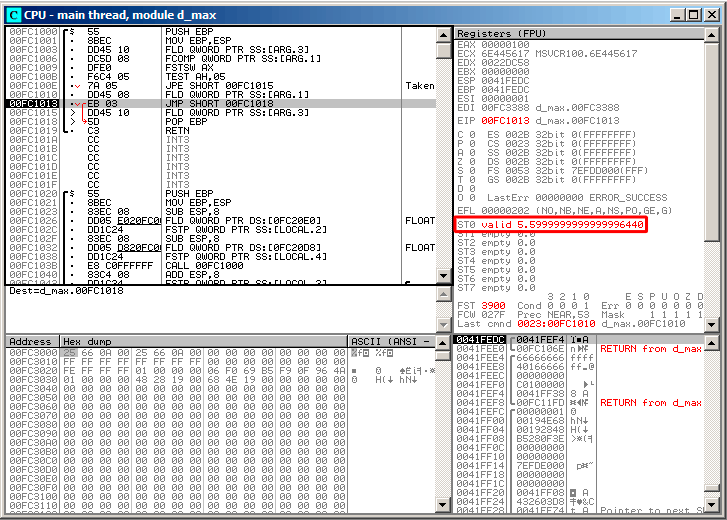
\includegraphics[scale=\FigScale]{patterns/12_FPU/3_comparison/x86/MSVC/olly2_5.png}
\caption{\olly: \RU{вторая \FLD исполнилась}\EN{second \FLD executed}}
\label{fig:FPU_comparison_case2_olly5}
\end{figure}
